% Created by tikzDevice version 0.12 on 2019-03-27 16:15:28
% !TEX encoding = UTF-8 Unicode
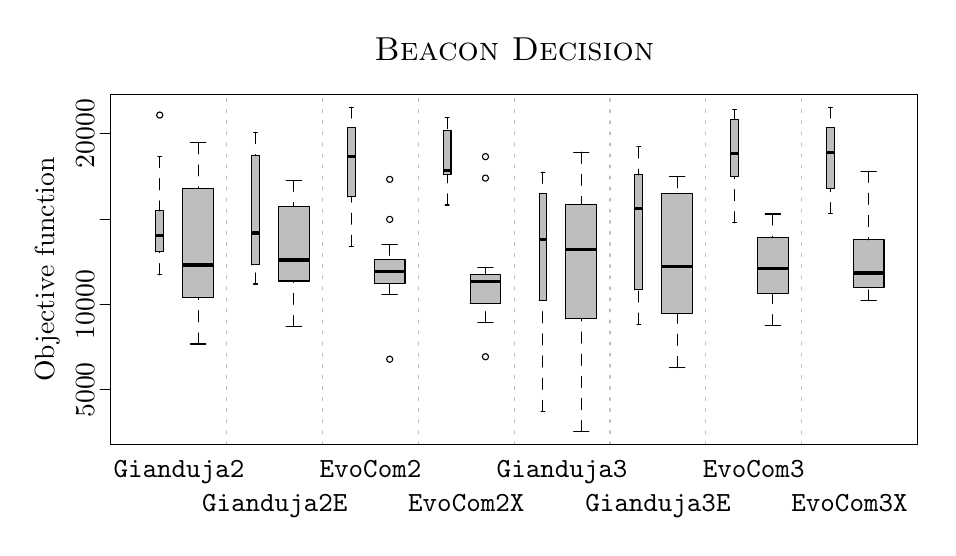
\begin{tikzpicture}[x=1pt,y=1pt]
\definecolor{fillColor}{RGB}{255,255,255}
\path[use as bounding box,fill=fillColor,fill opacity=0.00] (0,0) rectangle (325.21,180.67);
\begin{scope}
\path[clip] ( 30.00, 30.00) rectangle (321.61,156.67);
\definecolor{fillColor}{RGB}{190,190,190}

\path[fill=fillColor] ( 46.34, 99.69) --
	( 49.11, 99.69) --
	( 49.11,114.51) --
	( 46.34,114.51) --
	cycle;
\definecolor{drawColor}{RGB}{0,0,0}

\path[draw=drawColor,line width= 1.2pt,line join=round] ( 46.34,105.47) -- ( 49.11,105.47);

\path[draw=drawColor,line width= 0.4pt,dash pattern=on 4pt off 4pt ,line join=round,line cap=round] ( 47.72, 91.37) -- ( 47.72, 99.69);

\path[draw=drawColor,line width= 0.4pt,dash pattern=on 4pt off 4pt ,line join=round,line cap=round] ( 47.72,134.09) -- ( 47.72,114.51);

\path[draw=drawColor,line width= 0.4pt,line join=round,line cap=round] ( 47.03, 91.37) -- ( 48.42, 91.37);

\path[draw=drawColor,line width= 0.4pt,line join=round,line cap=round] ( 47.03,134.09) -- ( 48.42,134.09);

\path[draw=drawColor,line width= 0.4pt,line join=round,line cap=round] ( 46.34, 99.69) --
	( 49.11, 99.69) --
	( 49.11,114.51) --
	( 46.34,114.51) --
	( 46.34, 99.69);

\path[draw=drawColor,line width= 0.4pt,line join=round,line cap=round] ( 47.72,149.09) circle (  1.12);

\path[fill=fillColor] ( 56.03, 83.14) --
	( 67.11, 83.14) --
	( 67.11,122.62) --
	( 56.03,122.62) --
	cycle;

\path[draw=drawColor,line width= 1.2pt,line join=round] ( 56.03, 94.87) -- ( 67.11, 94.87);

\path[draw=drawColor,line width= 0.4pt,dash pattern=on 4pt off 4pt ,line join=round,line cap=round] ( 61.57, 66.38) -- ( 61.57, 83.14);

\path[draw=drawColor,line width= 0.4pt,dash pattern=on 4pt off 4pt ,line join=round,line cap=round] ( 61.57,139.11) -- ( 61.57,122.62);

\path[draw=drawColor,line width= 0.4pt,line join=round,line cap=round] ( 58.80, 66.38) -- ( 64.34, 66.38);

\path[draw=drawColor,line width= 0.4pt,line join=round,line cap=round] ( 58.80,139.11) -- ( 64.34,139.11);

\path[draw=drawColor,line width= 0.4pt,line join=round,line cap=round] ( 56.03, 83.14) --
	( 67.11, 83.14) --
	( 67.11,122.62) --
	( 56.03,122.62) --
	( 56.03, 83.14);

\path[fill=fillColor] ( 80.96, 95.00) --
	( 83.73, 95.00) --
	( 83.73,134.49) --
	( 80.96,134.49) --
	cycle;

\path[draw=drawColor,line width= 1.2pt,line join=round] ( 80.96,106.47) -- ( 83.73,106.47);

\path[draw=drawColor,line width= 0.4pt,dash pattern=on 4pt off 4pt ,line join=round,line cap=round] ( 82.34, 88.06) -- ( 82.34, 95.00);

\path[draw=drawColor,line width= 0.4pt,dash pattern=on 4pt off 4pt ,line join=round,line cap=round] ( 82.34,142.81) -- ( 82.34,134.49);

\path[draw=drawColor,line width= 0.4pt,line join=round,line cap=round] ( 81.65, 88.06) -- ( 83.03, 88.06);

\path[draw=drawColor,line width= 0.4pt,line join=round,line cap=round] ( 81.65,142.81) -- ( 83.03,142.81);

\path[draw=drawColor,line width= 0.4pt,line join=round,line cap=round] ( 80.96, 95.00) --
	( 83.73, 95.00) --
	( 83.73,134.49) --
	( 80.96,134.49) --
	( 80.96, 95.00);

\path[fill=fillColor] ( 90.65, 89.11) --
	(101.73, 89.11) --
	(101.73,115.99) --
	( 90.65,115.99) --
	cycle;

\path[draw=drawColor,line width= 1.2pt,line join=round] ( 90.65, 96.75) -- (101.73, 96.75);

\path[draw=drawColor,line width= 0.4pt,dash pattern=on 4pt off 4pt ,line join=round,line cap=round] ( 96.19, 72.65) -- ( 96.19, 89.11);

\path[draw=drawColor,line width= 0.4pt,dash pattern=on 4pt off 4pt ,line join=round,line cap=round] ( 96.19,125.49) -- ( 96.19,115.99);

\path[draw=drawColor,line width= 0.4pt,line join=round,line cap=round] ( 93.42, 72.65) -- ( 98.96, 72.65);

\path[draw=drawColor,line width= 0.4pt,line join=round,line cap=round] ( 93.42,125.49) -- ( 98.96,125.49);

\path[draw=drawColor,line width= 0.4pt,line join=round,line cap=round] ( 90.65, 89.11) --
	(101.73, 89.11) --
	(101.73,115.99) --
	( 90.65,115.99) --
	( 90.65, 89.11);

\path[fill=fillColor] (115.57,119.54) --
	(118.34,119.54) --
	(118.34,144.73) --
	(115.57,144.73) --
	cycle;

\path[draw=drawColor,line width= 1.2pt,line join=round] (115.57,134.00) -- (118.34,134.00);

\path[draw=drawColor,line width= 0.4pt,dash pattern=on 4pt off 4pt ,line join=round,line cap=round] (116.96,101.65) -- (116.96,119.54);

\path[draw=drawColor,line width= 0.4pt,dash pattern=on 4pt off 4pt ,line join=round,line cap=round] (116.96,151.98) -- (116.96,144.73);

\path[draw=drawColor,line width= 0.4pt,line join=round,line cap=round] (116.27,101.65) -- (117.65,101.65);

\path[draw=drawColor,line width= 0.4pt,line join=round,line cap=round] (116.27,151.98) -- (117.65,151.98);

\path[draw=drawColor,line width= 0.4pt,line join=round,line cap=round] (115.57,119.54) --
	(118.34,119.54) --
	(118.34,144.73) --
	(115.57,144.73) --
	(115.57,119.54);

\path[fill=fillColor] (125.27, 88.36) --
	(136.34, 88.36) --
	(136.34, 96.85) --
	(125.27, 96.85) --
	cycle;

\path[draw=drawColor,line width= 1.2pt,line join=round] (125.27, 92.67) -- (136.34, 92.67);

\path[draw=drawColor,line width= 0.4pt,dash pattern=on 4pt off 4pt ,line join=round,line cap=round] (130.81, 84.27) -- (130.81, 88.36);

\path[draw=drawColor,line width= 0.4pt,dash pattern=on 4pt off 4pt ,line join=round,line cap=round] (130.81,102.36) -- (130.81, 96.85);

\path[draw=drawColor,line width= 0.4pt,line join=round,line cap=round] (128.04, 84.27) -- (133.57, 84.27);

\path[draw=drawColor,line width= 0.4pt,line join=round,line cap=round] (128.04,102.36) -- (133.57,102.36);

\path[draw=drawColor,line width= 0.4pt,line join=round,line cap=round] (125.27, 88.36) --
	(136.34, 88.36) --
	(136.34, 96.85) --
	(125.27, 96.85) --
	(125.27, 88.36);

\path[draw=drawColor,line width= 0.4pt,line join=round,line cap=round] (130.81,125.85) circle (  1.12);

\path[draw=drawColor,line width= 0.4pt,line join=round,line cap=round] (130.81,111.39) circle (  1.12);

\path[draw=drawColor,line width= 0.4pt,line join=round,line cap=round] (130.81, 60.87) circle (  1.12);

\path[fill=fillColor] (150.19,127.59) --
	(152.96,127.59) --
	(152.96,143.50) --
	(150.19,143.50) --
	cycle;

\path[draw=drawColor,line width= 1.2pt,line join=round] (150.19,128.96) -- (152.96,128.96);

\path[draw=drawColor,line width= 0.4pt,dash pattern=on 4pt off 4pt ,line join=round,line cap=round] (151.58,116.60) -- (151.58,127.59);

\path[draw=drawColor,line width= 0.4pt,dash pattern=on 4pt off 4pt ,line join=round,line cap=round] (151.58,148.23) -- (151.58,143.50);

\path[draw=drawColor,line width= 0.4pt,line join=round,line cap=round] (150.88,116.60) -- (152.27,116.60);

\path[draw=drawColor,line width= 0.4pt,line join=round,line cap=round] (150.88,148.23) -- (152.27,148.23);

\path[draw=drawColor,line width= 0.4pt,line join=round,line cap=round] (150.19,127.59) --
	(152.96,127.59) --
	(152.96,143.50) --
	(150.19,143.50) --
	(150.19,127.59);

\path[fill=fillColor] (159.88, 81.09) --
	(170.96, 81.09) --
	(170.96, 91.34) --
	(159.88, 91.34) --
	cycle;

\path[draw=drawColor,line width= 1.2pt,line join=round] (159.88, 88.92) -- (170.96, 88.92);

\path[draw=drawColor,line width= 0.4pt,dash pattern=on 4pt off 4pt ,line join=round,line cap=round] (165.42, 74.04) -- (165.42, 81.09);

\path[draw=drawColor,line width= 0.4pt,dash pattern=on 4pt off 4pt ,line join=round,line cap=round] (165.42, 94.06) -- (165.42, 91.34);

\path[draw=drawColor,line width= 0.4pt,line join=round,line cap=round] (162.65, 74.04) -- (168.19, 74.04);

\path[draw=drawColor,line width= 0.4pt,line join=round,line cap=round] (162.65, 94.06) -- (168.19, 94.06);

\path[draw=drawColor,line width= 0.4pt,line join=round,line cap=round] (159.88, 81.09) --
	(170.96, 81.09) --
	(170.96, 91.34) --
	(159.88, 91.34) --
	(159.88, 81.09);

\path[draw=drawColor,line width= 0.4pt,line join=round,line cap=round] (165.42,126.30) circle (  1.12);

\path[draw=drawColor,line width= 0.4pt,line join=round,line cap=round] (165.42, 61.76) circle (  1.12);

\path[draw=drawColor,line width= 0.4pt,line join=round,line cap=round] (165.42,134.06) circle (  1.12);

\path[fill=fillColor] (184.81, 82.21) --
	(187.58, 82.21) --
	(187.58,120.76) --
	(184.81,120.76) --
	cycle;

\path[draw=drawColor,line width= 1.2pt,line join=round] (184.81,104.24) -- (187.58,104.24);

\path[draw=drawColor,line width= 0.4pt,dash pattern=on 4pt off 4pt ,line join=round,line cap=round] (186.19, 42.02) -- (186.19, 82.21);

\path[draw=drawColor,line width= 0.4pt,dash pattern=on 4pt off 4pt ,line join=round,line cap=round] (186.19,128.42) -- (186.19,120.76);

\path[draw=drawColor,line width= 0.4pt,line join=round,line cap=round] (185.50, 42.02) -- (186.88, 42.02);

\path[draw=drawColor,line width= 0.4pt,line join=round,line cap=round] (185.50,128.42) -- (186.88,128.42);

\path[draw=drawColor,line width= 0.4pt,line join=round,line cap=round] (184.81, 82.21) --
	(187.58, 82.21) --
	(187.58,120.76) --
	(184.81,120.76) --
	(184.81, 82.21);

\path[fill=fillColor] (194.50, 75.45) --
	(205.58, 75.45) --
	(205.58,116.71) --
	(194.50,116.71) --
	cycle;

\path[draw=drawColor,line width= 1.2pt,line join=round] (194.50,100.52) -- (205.58,100.52);

\path[draw=drawColor,line width= 0.4pt,dash pattern=on 4pt off 4pt ,line join=round,line cap=round] (200.04, 34.69) -- (200.04, 75.45);

\path[draw=drawColor,line width= 0.4pt,dash pattern=on 4pt off 4pt ,line join=round,line cap=round] (200.04,135.66) -- (200.04,116.71);

\path[draw=drawColor,line width= 0.4pt,line join=round,line cap=round] (197.27, 34.69) -- (202.81, 34.69);

\path[draw=drawColor,line width= 0.4pt,line join=round,line cap=round] (197.27,135.66) -- (202.81,135.66);

\path[draw=drawColor,line width= 0.4pt,line join=round,line cap=round] (194.50, 75.45) --
	(205.58, 75.45) --
	(205.58,116.71) --
	(194.50,116.71) --
	(194.50, 75.45);

\path[fill=fillColor] (219.43, 85.95) --
	(222.19, 85.95) --
	(222.19,127.52) --
	(219.43,127.52) --
	cycle;

\path[draw=drawColor,line width= 1.2pt,line join=round] (219.43,115.21) -- (222.19,115.21);

\path[draw=drawColor,line width= 0.4pt,dash pattern=on 4pt off 4pt ,line join=round,line cap=round] (220.81, 73.50) -- (220.81, 85.95);

\path[draw=drawColor,line width= 0.4pt,dash pattern=on 4pt off 4pt ,line join=round,line cap=round] (220.81,137.58) -- (220.81,127.52);

\path[draw=drawColor,line width= 0.4pt,line join=round,line cap=round] (220.12, 73.50) -- (221.50, 73.50);

\path[draw=drawColor,line width= 0.4pt,line join=round,line cap=round] (220.12,137.58) -- (221.50,137.58);

\path[draw=drawColor,line width= 0.4pt,line join=round,line cap=round] (219.43, 85.95) --
	(222.19, 85.95) --
	(222.19,127.52) --
	(219.43,127.52) --
	(219.43, 85.95);

\path[fill=fillColor] (229.12, 77.42) --
	(240.20, 77.42) --
	(240.20,120.82) --
	(229.12,120.82) --
	cycle;

\path[draw=drawColor,line width= 1.2pt,line join=round] (229.12, 94.34) -- (240.20, 94.34);

\path[draw=drawColor,line width= 0.4pt,dash pattern=on 4pt off 4pt ,line join=round,line cap=round] (234.66, 57.87) -- (234.66, 77.42);

\path[draw=drawColor,line width= 0.4pt,dash pattern=on 4pt off 4pt ,line join=round,line cap=round] (234.66,126.76) -- (234.66,120.82);

\path[draw=drawColor,line width= 0.4pt,line join=round,line cap=round] (231.89, 57.87) -- (237.43, 57.87);

\path[draw=drawColor,line width= 0.4pt,line join=round,line cap=round] (231.89,126.76) -- (237.43,126.76);

\path[draw=drawColor,line width= 0.4pt,line join=round,line cap=round] (229.12, 77.42) --
	(240.20, 77.42) --
	(240.20,120.82) --
	(229.12,120.82) --
	(229.12, 77.42);

\path[fill=fillColor] (254.04,126.83) --
	(256.81,126.83) --
	(256.81,147.60) --
	(254.04,147.60) --
	cycle;

\path[draw=drawColor,line width= 1.2pt,line join=round] (254.04,135.26) -- (256.81,135.26);

\path[draw=drawColor,line width= 0.4pt,dash pattern=on 4pt off 4pt ,line join=round,line cap=round] (255.43,110.17) -- (255.43,126.83);

\path[draw=drawColor,line width= 0.4pt,dash pattern=on 4pt off 4pt ,line join=round,line cap=round] (255.43,151.15) -- (255.43,147.60);

\path[draw=drawColor,line width= 0.4pt,line join=round,line cap=round] (254.73,110.17) -- (256.12,110.17);

\path[draw=drawColor,line width= 0.4pt,line join=round,line cap=round] (254.73,151.15) -- (256.12,151.15);

\path[draw=drawColor,line width= 0.4pt,line join=round,line cap=round] (254.04,126.83) --
	(256.81,126.83) --
	(256.81,147.60) --
	(254.04,147.60) --
	(254.04,126.83);

\path[fill=fillColor] (263.74, 84.63) --
	(274.81, 84.63) --
	(274.81,104.76) --
	(263.74,104.76) --
	cycle;

\path[draw=drawColor,line width= 1.2pt,line join=round] (263.74, 93.53) -- (274.81, 93.53);

\path[draw=drawColor,line width= 0.4pt,dash pattern=on 4pt off 4pt ,line join=round,line cap=round] (269.27, 72.98) -- (269.27, 84.63);

\path[draw=drawColor,line width= 0.4pt,dash pattern=on 4pt off 4pt ,line join=round,line cap=round] (269.27,113.34) -- (269.27,104.76);

\path[draw=drawColor,line width= 0.4pt,line join=round,line cap=round] (266.50, 72.98) -- (272.04, 72.98);

\path[draw=drawColor,line width= 0.4pt,line join=round,line cap=round] (266.50,113.34) -- (272.04,113.34);

\path[draw=drawColor,line width= 0.4pt,line join=round,line cap=round] (263.74, 84.63) --
	(274.81, 84.63) --
	(274.81,104.76) --
	(263.74,104.76) --
	(263.74, 84.63);

\path[fill=fillColor] (288.66,122.70) --
	(291.43,122.70) --
	(291.43,144.73) --
	(288.66,144.73) --
	cycle;

\path[draw=drawColor,line width= 1.2pt,line join=round] (288.66,135.60) -- (291.43,135.60);

\path[draw=drawColor,line width= 0.4pt,dash pattern=on 4pt off 4pt ,line join=round,line cap=round] (290.04,113.47) -- (290.04,122.70);

\path[draw=drawColor,line width= 0.4pt,dash pattern=on 4pt off 4pt ,line join=round,line cap=round] (290.04,151.98) -- (290.04,144.73);

\path[draw=drawColor,line width= 0.4pt,line join=round,line cap=round] (289.35,113.47) -- (290.74,113.47);

\path[draw=drawColor,line width= 0.4pt,line join=round,line cap=round] (289.35,151.98) -- (290.74,151.98);

\path[draw=drawColor,line width= 0.4pt,line join=round,line cap=round] (288.66,122.70) --
	(291.43,122.70) --
	(291.43,144.73) --
	(288.66,144.73) --
	(288.66,122.70);

\path[fill=fillColor] (298.35, 86.83) --
	(309.43, 86.83) --
	(309.43,103.97) --
	(298.35,103.97) --
	cycle;

\path[draw=drawColor,line width= 1.2pt,line join=round] (298.35, 92.07) -- (309.43, 92.07);

\path[draw=drawColor,line width= 0.4pt,dash pattern=on 4pt off 4pt ,line join=round,line cap=round] (303.89, 81.93) -- (303.89, 86.83);

\path[draw=drawColor,line width= 0.4pt,dash pattern=on 4pt off 4pt ,line join=round,line cap=round] (303.89,128.82) -- (303.89,103.97);

\path[draw=drawColor,line width= 0.4pt,line join=round,line cap=round] (301.12, 81.93) -- (306.66, 81.93);

\path[draw=drawColor,line width= 0.4pt,line join=round,line cap=round] (301.12,128.82) -- (306.66,128.82);

\path[draw=drawColor,line width= 0.4pt,line join=round,line cap=round] (298.35, 86.83) --
	(309.43, 86.83) --
	(309.43,103.97) --
	(298.35,103.97) --
	(298.35, 86.83);
\definecolor{drawColor}{RGB}{190,190,190}

\path[draw=drawColor,line width= 0.4pt,dash pattern=on 1pt off 3pt ,line join=round,line cap=round] ( 71.96, 30.00) -- ( 71.96,156.67);

\path[draw=drawColor,line width= 0.4pt,dash pattern=on 1pt off 3pt ,line join=round,line cap=round] (106.57, 30.00) -- (106.57,156.67);

\path[draw=drawColor,line width= 0.4pt,dash pattern=on 1pt off 3pt ,line join=round,line cap=round] (141.19, 30.00) -- (141.19,156.67);

\path[draw=drawColor,line width= 0.4pt,dash pattern=on 1pt off 3pt ,line join=round,line cap=round] (175.81, 30.00) -- (175.81,156.67);

\path[draw=drawColor,line width= 0.4pt,dash pattern=on 1pt off 3pt ,line join=round,line cap=round] (210.42, 30.00) -- (210.42,156.67);

\path[draw=drawColor,line width= 0.4pt,dash pattern=on 1pt off 3pt ,line join=round,line cap=round] (245.04, 30.00) -- (245.04,156.67);

\path[draw=drawColor,line width= 0.4pt,dash pattern=on 1pt off 3pt ,line join=round,line cap=round] (279.66, 30.00) -- (279.66,156.67);
\end{scope}
\begin{scope}
\path[clip] (  0.00,  0.00) rectangle (325.21,180.67);
\definecolor{drawColor}{RGB}{0,0,0}

\node[text=drawColor,anchor=base,inner sep=0pt, outer sep=0pt, scale=  1.00] at ( 54.65, 18.00) {\texttt{Gianduja2}};

\node[text=drawColor,anchor=base,inner sep=0pt, outer sep=0pt, scale=  1.00] at (123.88, 18.00) {\texttt{EvoCom2}};

\node[text=drawColor,anchor=base,inner sep=0pt, outer sep=0pt, scale=  1.00] at (193.12, 18.00) {\texttt{Gianduja3}};

\node[text=drawColor,anchor=base,inner sep=0pt, outer sep=0pt, scale=  1.00] at (262.35, 18.00) {\texttt{EvoCom3}};

\node[text=drawColor,anchor=base,inner sep=0pt, outer sep=0pt, scale=  1.00] at ( 89.26,  6.00) {\texttt{Gianduja2E}};

\node[text=drawColor,anchor=base,inner sep=0pt, outer sep=0pt, scale=  1.00] at (158.50,  6.00) {\texttt{EvoCom2X}};

\node[text=drawColor,anchor=base,inner sep=0pt, outer sep=0pt, scale=  1.00] at (227.73,  6.00) {\texttt{Gianduja3E}};

\node[text=drawColor,anchor=base,inner sep=0pt, outer sep=0pt, scale=  1.00] at (296.97,  6.00) {\texttt{EvoCom3X}};
\end{scope}
\begin{scope}
\path[clip] (  0.00,  0.00) rectangle (325.21,180.67);
\definecolor{drawColor}{RGB}{0,0,0}

\node[text=drawColor,anchor=base,inner sep=0pt, outer sep=0pt, scale=  1.20] at (175.81,168.67) {\textsc{Beacon Decision}};

\node[text=drawColor,rotate= 90.00,anchor=base,inner sep=0pt, outer sep=0pt, scale=  1.00] at (  9.60, 93.34) {Objective function};
\end{scope}
\begin{scope}
\path[clip] (  0.00,  0.00) rectangle (325.21,180.67);
\definecolor{drawColor}{RGB}{0,0,0}

\path[draw=drawColor,line width= 0.4pt,line join=round,line cap=round] ( 30.00, 49.80) -- ( 30.00,142.34);

\path[draw=drawColor,line width= 0.4pt,line join=round,line cap=round] ( 30.00, 49.80) -- ( 26.20, 49.80);

\path[draw=drawColor,line width= 0.4pt,line join=round,line cap=round] ( 30.00, 80.65) -- ( 26.20, 80.65);

\path[draw=drawColor,line width= 0.4pt,line join=round,line cap=round] ( 30.00,111.49) -- ( 26.20,111.49);

\path[draw=drawColor,line width= 0.4pt,line join=round,line cap=round] ( 30.00,142.34) -- ( 26.20,142.34);

\node[text=drawColor,rotate= 90.00,anchor=base,inner sep=0pt, outer sep=0pt, scale=  1.00] at ( 24.00, 49.80) {5000};

\node[text=drawColor,rotate= 90.00,anchor=base,inner sep=0pt, outer sep=0pt, scale=  1.00] at ( 24.00, 80.65) {10000};

\node[text=drawColor,rotate= 90.00,anchor=base,inner sep=0pt, outer sep=0pt, scale=  1.00] at ( 24.00,142.34) {20000};

\path[draw=drawColor,line width= 0.4pt,line join=round,line cap=round] ( 30.00, 30.00) --
	(321.61, 30.00) --
	(321.61,156.67) --
	( 30.00,156.67) --
	( 30.00, 30.00);
\end{scope}
\end{tikzpicture}
